\ylDisplay{Jope} % Ülesande nimi
{Andres Põldaru} % Autor
{piirkonnavoor} % Voor
{2019} % Aasta
{P 3} % Ülesande nr.
{2} % Raskustase
{
% Teema: Valgusõpetus
\ifStatement
Juku tahab peeglist vaadata, kuidas talle uus jope selga sobib. Peegel on aga väike ja sealt paistab ainult pool jopet. Põhjendage, kas peeglile lähemale/kaugemale minnes on jopet rohkem näha. 
\fi
\ifHint
Ülesande lahenduse paremaks selgitamiseks on mõistlik teha joonis.
\fi
\ifSolution
Et vastata küsimusele, kas kaugemalt/lähemalt vaadates on peeglis rohkem jopet näha uurime, millises seoses on peeglis vaadeldava eseme ja peegli kõrgus. \\
Eeldame, et inimene $AD$ ja peegel $KL$ paiknevad mõlemad vertikaalselt ning inimese silm asub punktis A. 
Asugu peegli ülemine äär inimese silmaga samal kõrgusel. Sel juhul näeb inimene peegli ülemises servas oma silma. Peegli alumises servas näeb ta oma keha punkti $C$. 
Vastavalt peegeldumise seadusele on valguse peegeldumisnurk $ALB$ võrdne langemisnurgaga $BLC$. 
Seega saame väita, et kolmnurk $ABL$ ja kolmnurk $CLB$ on võrdsed, sest neil on ühine kattuv külg $LB$ ja mõlema kolmnurga ühise külje lähisnurgad on võrdsed. Üks külje $LB$ lähisnurkadest on vastavalt kas valguse langemis- või peegeldumisnurk kolmnurkade tipu $L$ juures ja teine täisnurk kolmnurkade tipu $B$ juures. 
Seega lõigud $AB$ ja $CB$ kui kolmnurkade vastavad küljed on suuruselt võrdsed. 
Kuna lõik $AB$ on võrdne peegli kõrgusega $KL$, on peeglis nähtav ese, mis on kaks korda kõrgem peegli kõrgusest.
Võib teha teise joonise, kus inimene asub kaugemal või lähemal peeglile. Kui vaadeldav ese ja peegel asuvad paralleelselt, on sõltumata eseme kaugusest peeglist peeglis nähtava eseme kõrgus võrdne peegli kahekordse kõrgusega. Seega ei näe Juku sellest peeglist tervet jopet ka siis, kui astub peeglile lähemale või eemaldub peeglist. 
Märkus: kui jope ja silmad pole peeglist sama kaugel, siis sõltuvalt täpsest objektide asetusest võib lähemale minnes nii rohkem kui ka vähem jopet näha olla.
\begin{center}
	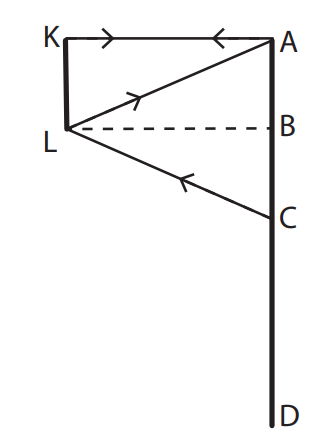
\includegraphics[width=0.5\linewidth]{2019-v2p-03-lah.PNG}
\end{center}
\fi
}
